\documentclass[11pt,a4paper]{article}
\usepackage[margin=25mm]{geometry}
\usepackage[T1]{fontenc}
\usepackage{lmodern}
\usepackage{graphicx,booktabs,amsmath,amssymb}
\usepackage{enumitem,caption,placeins}
\usepackage[hidelinks]{hyperref}
\graphicspath{{figures/}}
\linespread{1.18}
\setcounter{tocdepth}{2}
\setlength{\parindent}{0pt}
\setlength{\parskip}{5pt}
\setlength{\emergencystretch}{2em}
\setlist[itemize]{leftmargin=1.5em,itemsep=4pt,topsep=4pt}
\captionsetup{font=small,labelfont=bf}
\renewcommand{\topfraction}{0.9}
\renewcommand{\bottomfraction}{0.8}
\renewcommand{\textfraction}{0.1}
\renewcommand{\floatpagefraction}{0.85}
\newcommand{\sectionauthor}{\noindent\textit{Section author: [to be completed]}\par\vspace{3pt}}
\title{\textbf{Multi-Step Forecasting of Electricity Demand\protect\\and Solar Power Generation}\protect\\[8pt]
\large ELEN90099 Deep Learning\protect\\Learn--Design--Implement Project: Draft Report}
\author{Student 1: [Name and student ID]\protect\\Student 2: [Name and student ID]}
\date{October 2026}
\begin{document}
\hypersetup{pageanchor=false}
\begin{titlepage}
\maketitle\thispagestyle{empty}
\vfill
\begin{center}\begin{minipage}{0.85\textwidth}
\textbf{Draft status.} The introduction and project scope are developed; later sections combine initial findings with concise design notes and planned work. Author details and actual section responsibilities must be completed before submission.
\end{minipage}\end{center}
\end{titlepage}
\pagenumbering{roman}\hypersetup{pageanchor=true}
\tableofcontents\clearpage\pagenumbering{arabic}
% Two-student body target: 8--10 pages, excluding title, contents and references.
% Suggested allocation: Introduction 15%, Problem 35%, Experiments 35%, Conclusion 15%.

\section{Introduction}\label{sec:introduction}
\sectionauthor
\subsection{Overview and Background}
Electricity demand and solar generation vary over time, creating a need for forecasts when planning energy supply and storage. A forecast of the next day's trajectory is more informative than a single next-step estimate because it describes when demand or output may rise and fall. However, a forecasting model must also recognise the limits of its information. Historical observations can reveal recurring patterns, but cannot directly provide future weather conditions or explain every unusual event.

This project studies two separate tasks: hourly electricity demand and ten-minute solar output. Both use the most recent 48 hours to predict the following 24 hours. We train a separate model for each dataset and evaluate 16 fixed channels per task. The Monash archive provides accessible forecasting benchmarks with different temporal characteristics~\cite{monash}. Using the same history duration and forecast duration allows us to examine how model behaviour changes between two energy-related tasks while keeping the experimental question manageable.

Our aim is to investigate whether deep learning adds useful predictive accuracy beyond simple daily repetition, and whether that benefit justifies a larger model. At this stage, the project concerns supervised forecasting, rather than electricity dispatch or storage control. The report presents initial experiments and a plan for further validation; prediction errors alone do not establish operational or financial benefits.

\subsection{Literature Overview and State of the Art}
The selected literature represents several approaches to sequence modelling. LSTM introduces gated memory, while GRU uses a simpler gated recurrent state~\cite{lstm,gru}. Temporal convolution provides a complementary way to detect local patterns. These mechanisms motivate comparing recurrence, convolution and their combination on the same forecasting task.

Recent forecasting work also questions whether increasing architectural complexity necessarily improves accuracy. Zeng et al. introduce simple linear models, including a decomposition-based approach, as competitive alternatives to more complicated forecasting networks~\cite{dlinear}. Nie et al. propose PatchTST, using temporal patches and shared channel-independent processing~\cite{patch}. Together, these studies motivate testing both a lightweight DLinear implementation and a patch-attention model. They do not imply that the same ranking will hold on our subsets or under our short training budget.

The literature review in this draft is intentionally focused on the methods used in the project. The local attention model is inspired by PatchTST but is not an exact reproduction of the published implementation. Published benchmark results therefore provide design motivation, rather than scores directly comparable with our experiments.

\subsection{Project Scope and Tasks}
The project asks three questions. First, do trainable models improve on persistence and daily seasonal naive prediction? Second, how do recurrent, convolutional, hybrid, linear and attention-based models differ in accuracy and computational cost? Third, do conclusions change when evaluating difficult output conditions or varying the available history and training data?

The tasks are to prepare fixed subsets, define a common evaluation protocol, implement the model families, and compare initial results. Inputs contain historical target observations only; weather forecasts, calendar features and future observations are excluded. This restriction clarifies what is being learned, while limiting the ability to anticipate events absent from the history. The draft follows the course's intended progression from problem formulation to initial experiments and further work~\cite{course}.

\FloatBarrier
\section{Problem Definition and Scope}\label{sec:problem}
\sectionauthor
\subsection{Problem Definition and Forecasting Task}
The task is direct multi-step regression. Let $X\in\mathbb{R}^{T\times C}$ contain $T$ observations across $C=16$ channels. At origin $t$, a model receives the historical window and estimates the complete future target:
\begin{equation}\label{eq:task}
\widehat{Y}_{t}=f_{\theta}(X_{t-L:t})\in\mathbb{R}^{H\times C},
\qquad Y_t=X_{t:t+H}.
\end{equation}
The slices are half-open: the input ends at $t-1$, and the target begins at $t$. Table~\ref{tab:data} specifies the step counts for the common 48-hour history and 24-hour horizon. Every model predicts all channels and future steps in one forward pass, rather than recursively using its own predictions as later inputs.

\begin{itemize}
\item \textbf{Available information:} only observations already revealed at the forecast origin. The 16 channels may be processed jointly or independently, depending on the model.
\item \textbf{Evaluation setting:} rolling origins move forward through the test interval. A later origin can use newly observed values, so this is not one frozen forecast made at the start of the test period.
\item \textbf{Intended outcome:} reliable comparisons on the chosen subsets, with errors measured in the original release scale and relative to a training-based seasonal reference.
\end{itemize}
The same protocol is more important than giving every architecture the same number of layers. Different designs use different representations and parameter counts; these differences are part of the comparison and must be considered when interpreting results.

\subsection{Relevant Datasets and Preprocessing}
The Electricity Hourly and Solar 10 Minutes files come from the original Monash-linked releases~\cite{electricity,solar}. Electricity contains 321 hourly series; Solar contains 137 ten-minute series. The Solar release derives from a simulated PV source, so it should not be described as a field deployment dataset. The project selects 16 aligned channels from each release. These are separate datasets, not matched observations of one energy system.

\begin{table}[htbp]
\centering\small\linespread{1.1}\selectfont
\ifdefined\ChineseReport
\caption{数据集与预测任务概况。两个数据集分别建模，均使用 48 小时历史预测未来 24 小时。}
\else
\caption{Datasets and forecasting tasks. Models are fitted separately; both tasks use 48 hours of history to predict the next 24 hours.}
\fi
\label{tab:data}
\begin{tabular}{lrr}
\toprule
\ifdefined\ChineseReport
属性 & Electricity & Solar\\
\midrule
发布序列数 / 选用通道数 & 321 / 16 & 137 / 16\\
每条序列的样本数 & 26,304 & 52,560\\
采样间隔 & 1 小时 & 10 分钟\\
数据年份 & 2012--2014 & 2006\\
历史窗口 $L$（步） & 48 & 288\\
预测时域 $H$（步） & 24 & 144\\
日周期 $m$（步） & 24 & 144\\
训练区间零值占比 & 0.0\% & 53.0\%\\
\else
Property & Electricity & Solar\\
\midrule
Source series / selected channels & 321 / 16 & 137 / 16\\
Samples per series & 26,304 & 52,560\\
Sampling interval & 1 hour & 10 minutes\\
Source years & 2012--2014 & 2006\\
History $L$ (steps) & 48 & 288\\
Horizon $H$ (steps) & 24 & 144\\
Daily period $m$ (steps) & 24 & 144\\
Zero values in training & 0.0\% & 53.0\%\\
\fi
\bottomrule
\end{tabular}
\end{table}


Selection is fixed before the reported comparisons. Using training-period means, source series are sorted into four scale groups and four series are sampled from each group with seed 42. This gives a range of average magnitudes without using test performance to choose channels. It does not establish that 16 series represent the full population. The selected IDs and data checks are retained with the experiment records.

Figure~\ref{fig:data} shows the first seven days of the first selected channel and the training-period channel correlations. Daily structure motivates the seasonal baseline. The high Solar zero-value proportion also motivates evaluating active output separately, because a low full-period error can conceal differences during periods of larger generation. Correlation suggests shared variation but does not prove that modelling interactions between channels will improve predictions.

\begin{figure}[htbp]
\centering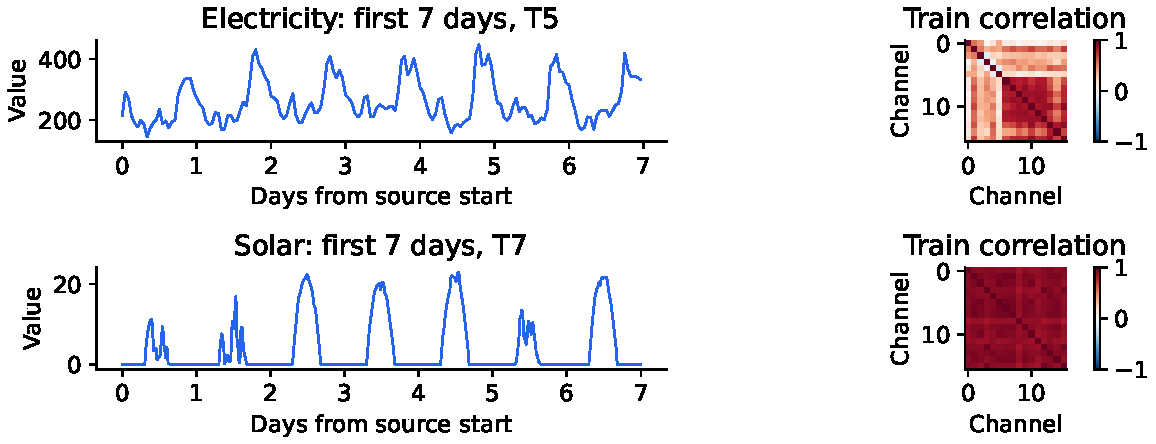
\includegraphics[width=\textwidth,height=7cm,keepaspectratio]{data_overview.pdf}
\caption{Data overview from the fixed subsets: the first seven source days for channels T5 and T7, with correlations computed on training data only. Values retain the original release scale.}
\label{fig:data}
\end{figure}

Preprocessing uses per-channel means and standard deviations fitted only on the training interval. Validation and test inputs use those fixed statistics, and predictions are transformed back before computing errors. No interpolation or unit conversion is applied. Since the aggregate releases' physical units have not been independently resolved in the experiment records, plots and errors are reported in original release units. The source time grid is retained without assigning an unverified local timezone.

\subsection{Approach and Deep Learning Models}
The implementation uses a shared forecasting interface with two non-learning baselines and six trainable models. The baselines are described in Section~\ref{sec:alternatives}; the deep learning designs are summarised here.
\begin{itemize}
\item \textbf{LSTM and GRU:} one recurrent layer with hidden size 64 receives all channels at each step. The final hidden state is projected to the full $H\times C$ output. GRU provides a simpler gated comparison with fewer recurrent parameters.
\item \textbf{1D-CNN:} two temporal convolutions of width three use 32 and 64 feature channels, batch normalisation and ReLU. Adaptive average pooling to 16 positions feeds a dense multi-step head.
\item \textbf{CNN--LSTM:} a width-three convolution creates 64 features, followed by a 64-unit LSTM and dense output head. The design tests whether local feature extraction helps recurrent encoding.
\item \textbf{DLinear:} a 25-step moving average separates a smooth component and a remainder. Two learned linear maps project these components to the forecast horizon; the maps are shared across channels.
\item \textbf{PatchTST-style:} each channel is split into patches of length 16 and stride eight. A 64-dimensional embedding, two Transformer encoder layers and a linear head produce its forecast; weights are shared across channels.
\end{itemize}
The attention implementation uses four heads, feed-forward width 128, dropout 0.1 and learned positions. It uses training-set scaling and does not implement the original model's full normalisation pipeline. Both modern models are self-written implementations of selected ideas. The study therefore compares these concrete designs, rather than claiming to reproduce every published variant.

\subsection{Theoretical Foundations and Design Rationale}
The model choices connect course concepts to the structure of the task. The following points state the reasoning to be tested, rather than assumptions that the results already prove.
\begin{itemize}
\item \textbf{Memory and compression:} recurrent gates can retain useful historical information, but representing an entire window through the final state creates a compression bottleneck. This may matter more for Solar's 144-step output than for Electricity's 24-step output.
\item \textbf{Local feature sharing:} convolution reuses filters across time. The two width-three convolutions have a five-step local receptive field before pooling. Pooling aggregates the observed history; it does not make the network a dilated temporal convolutional model.
\item \textbf{Combining mechanisms:} the hybrid may extract local changes before recurrence. Its comparison with LSTM also changes input representation and capacity, so it is not an isolated ablation of convolution.
\item \textbf{Decomposition and attention:} DLinear imposes a simple separation of smooth and residual variation. Patching reduces the number of attention tokens. The residual need not be a pure seasonal component, and attention weights alone do not explain physical causes.
\end{itemize}
Equal settings in steps are not equal settings in physical time. A 25-step average spans 25 hours for Electricity but 4 hours 10 minutes for Solar. A 16-step patch spans 16 hours versus 2 hours 40 minutes. These differences may affect rankings and should be investigated before attributing results solely to model families. Channel-independent processing also provides a useful contrast to the jointly processed inputs of recurrent and convolutional models.

\FloatBarrier
\section{Experiments}\label{sec:experiments}
\sectionauthor
\subsection{Experimental Setup}
The initial experiments use one common protocol within each dataset. The settings below describe completed runs; longer training and additional controls remain planned work.
\begin{itemize}
\item \textbf{Temporal split:} the first 70\% of observations form training, the next 10\% validation, and the last 20\% test. Every target window must fit within its own interval. Historical input can extend into an earlier interval because it has already been observed.
\item \textbf{Forecast origins:} training windows advance by three hours, while validation and test windows advance by one hour. All main models use the same origins. This produces 5,238 test origins for Electricity and 1,729 for Solar.
\item \textbf{Training:} Adam, learning rate $10^{-3}$, weight decay $10^{-4}$, batch size 32, maximum five epochs and early-stopping patience three. Standardised MSE is the training loss, and the lowest validation-MSE checkpoint is evaluated.
\item \textbf{Replication and environment:} trainable main comparisons use seeds 42, 43 and 44 on an NVIDIA GeForce RTX 3060 Laptop GPU, with PyTorch 2.5.1+cu121. These are local GPU measurements, not measured Colab T4 results.
\end{itemize}
MAE measures average absolute error; RMSE gives larger errors more weight. Seasonal MASE divides each channel's MAE by its mean absolute daily difference in training, then averages across channels~\cite{mase}. The seasonal period is 24 steps for Electricity and 144 for Solar. A MASE below one refers to that training-based scale; beating the daily naive model on the test interval must be checked separately. Scores from the two datasets are not numerically comparable in absolute units.

Checkpoints, predictions, configurations and metrics are saved by run, with SQLite experiment records. Existing verification records report recomputation of metrics and checkpoint reload checks across 72 runs. These checks support consistency of the saved experiment, rather than establish generalisation. No new training is required to assemble this draft.

\subsection{Preliminary Results and Validation}
Table~\ref{tab:results} reports the main comparisons. Trainable-model values are means and sample standard deviations over three seeds. Persistence and daily naive are deterministic: repeating their records does not create independent forecasting trials. The standard deviations describe training variability, not confidence intervals over independent test days.

% Generated from my_report/submission/report/main_results.csv.
\begin{table}[htbp]
\centering\small\linespread{1.1}\selectfont
\setlength{\tabcolsep}{4pt}
\ifdefined\ChineseReport
\caption{初步测试结果（各数据集每项指标的最低均值加粗）。可训练模型为三个种子的均值 $\pm$ 样本标准差；确定性基线仅列数值。}
\else
\caption{Initial test results; lowest means per dataset and metric are bold. Trainable models: mean $\pm$ SD over three seeds; deterministic baselines: single values.}
\fi
\label{tab:results}
\begin{tabular}{lrrr}
\toprule
Model & MAE & RMSE & MASE\\
\midrule
\multicolumn{4}{l}{\textbf{Electricity}}\\
Persistence & 1,010.261 & 3,091.327 & 3.630\\
Daily naive & 208.218 & 732.211 & 1.009\\
LSTM & 262.727 $\pm$ 4.543 & 727.287 $\pm$ 15.818 & 1.310 $\pm$ 0.015\\
GRU & 262.592 $\pm$ 0.622 & 729.598 $\pm$ 2.779 & 1.304 $\pm$ 0.004\\
1D-CNN & 254.754 $\pm$ 1.493 & 696.794 $\pm$ 17.507 & 1.248 $\pm$ 0.026\\
CNN--LSTM & 267.183 $\pm$ 2.918 & 749.218 $\pm$ 9.099 & 1.310 $\pm$ 0.009\\
DLinear & 220.049 $\pm$ 0.504 & 665.572 $\pm$ 0.484 & 1.032 $\pm$ 0.003\\
PatchTST-style & \textbf{\boldmath 203.137 $\pm$ 3.301} & \textbf{\boldmath 636.246 $\pm$ 6.630} & \textbf{\boldmath 0.959 $\pm$ 0.012}\\
\midrule
\multicolumn{4}{l}{\textbf{Solar}}\\
Persistence & 7.379 & 12.546 & 3.048\\
Daily naive & \textbf{\boldmath 2.198} & 5.712 & \textbf{\boldmath 0.900}\\
LSTM & 3.653 $\pm$ 0.079 & 6.169 $\pm$ 0.192 & 1.493 $\pm$ 0.033\\
GRU & 3.665 $\pm$ 0.131 & 6.126 $\pm$ 0.175 & 1.498 $\pm$ 0.055\\
1D-CNN & 3.020 $\pm$ 0.045 & \textbf{\boldmath 4.888 $\pm$ 0.056} & 1.231 $\pm$ 0.018\\
CNN--LSTM & 3.462 $\pm$ 0.082 & 5.930 $\pm$ 0.146 & 1.414 $\pm$ 0.034\\
DLinear & 3.177 $\pm$ 0.037 & 5.236 $\pm$ 0.017 & 1.298 $\pm$ 0.015\\
PatchTST-style & 3.062 $\pm$ 0.036 & 5.100 $\pm$ 0.058 & 1.249 $\pm$ 0.015\\
\bottomrule
\end{tabular}
\end{table}


For Electricity, PatchTST-style obtains MAE 203.137, RMSE 636.246 and MASE 0.959, compared with daily naive's 208.218, 732.211 and 1.009. DLinear improves RMSE over daily naive, but has higher MAE and MASE. Thus an improvement in one metric should not be described as an improvement in every aspect of forecasting.

For Solar, daily naive has the lowest overall MAE (2.198) and MASE (0.900), whereas 1D-CNN has the lowest RMSE (4.888). This difference suggests that the methods distribute their errors differently. The five-epoch budget is insufficient to conclude that neural models are generally unsuitable for Solar. Further validation should establish whether the ranking survives fuller training.

\FloatBarrier
\subsection{Comparison of Deep Learning Models}
The preliminary comparison suggests different trade-offs for the two tasks:
\begin{itemize}
\item \textbf{Electricity:} PatchTST-style is strongest on the three overall metrics in this comparison. LSTM, GRU and CNN--LSTM do not consistently improve on daily naive. This is evidence about the current designs and training budget, not a general ranking of sequence-model families.
\item \textbf{Solar:} 1D-CNN has the best overall RMSE, while attention and decomposition remain competitive among trainable designs. A model that reduces large deviations can still have a higher average absolute error than a baseline that preserves repeated daily profiles.
\item \textbf{Resources:} Electricity DLinear has 2,352 parameters versus 76,056 for PatchTST-style. Their measured mean training times are about 3.0 and 9.4 seconds; mean per-run median forward latencies are about 0.52 and 1.52 ms. These are model-only local GPU measurements, not complete deployment latency.
\end{itemize}
Training time includes validation. The latency measurement uses inputs already on the device, ten warmups and 30 synchronised repetitions. Model size and these timings inform an initial accuracy--cost discussion, but do not determine embedded feasibility. Capacity, operator support and the larger Solar output head also affect resource use.

\subsection{Alternative Methods and Baseline Comparisons}\label{sec:alternatives}
Persistence repeats the latest observation for every future step. Daily seasonal naive repeats the latest observed day at the corresponding phase. Both use the same historical information as the networks and require no fitted parameters. Since each horizon is one day, the seasonal baseline does not need observations beyond the available input.

Both baselines are already evaluated, rather than proposed future alternatives. Daily naive is substantially stronger than persistence on both datasets. On Solar it is the most effective current choice if overall MAE or MASE is the primary objective. On Electricity its closeness to the best trainable model makes it a useful reference when judging whether added complexity is worthwhile.

A pretrained forecasting foundation model is an optional future comparison only. No such model has been run in the current project. Any extension would need to preserve the fixed subsets, origins and information restrictions, and document whether pretraining changes the basis of comparison. It is not required for completing the planned final-report experiments.

\subsection{Discussion and Interpretation}
Figure~\ref{fig:cases} illustrates difficult cases selected by a fixed rule: use the first chosen channel and select the earliest forecast window containing its largest true test target. Seed 42 is fixed; no model's error or best seed is used to choose the example. These cases show amplitude and timing mismatches but are stress illustrations, not representative samples of all forecasts.

\begin{figure}[htbp]
\centering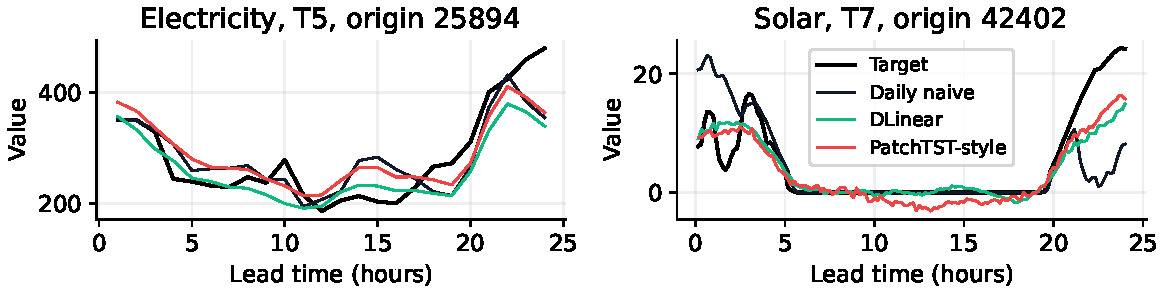
\includegraphics[width=\textwidth,height=6cm,keepaspectratio]{hard_cases.pdf}
\caption{Fixed-rule difficult forecasts for Electricity T5 (origin 25,894) and Solar T7 (origin 42,402), using seed 42. The cases are selected by true peak output rather than by a model's prediction error.}
\label{fig:cases}
\end{figure}
\FloatBarrier

\begin{itemize}
\item \textbf{Conditional errors:} Solar active output is defined as true output at least 10\% of a channel's training maximum. PatchTST-style and DLinear have active-output MAE 4.871 and 4.896, below daily naive's 5.655, despite worse full-period MAE. This mask is an evaluation condition, not a verified daylight label or an input feature.
\item \textbf{Sensitivity completed so far:} LSTM and PatchTST-style were tested with 24/48/168-hour histories and 25/50/100\% of the training interval, using seed 42 only. History comparisons use common origins. Results do not establish a universal monotonic benefit; longer histories also change attention capacity, while data fractions change recency, seasonal coverage and optimiser updates.
\item \textbf{Interpretation limits:} hourly rolling windows overlap, so test errors are dependent. The existing test interval has already been inspected during project development. It should not be described as an untouched external blind test, and no independent-window significance claim is made.
\end{itemize}
Raw negative predictions remain in the main scores. Uniform clipping can be studied later as a separate post-processing comparison. A broader analysis of lead times and channel-specific errors is reserved for the final report, with attention to whether apparent improvements concern the conditions that matter for the task.

\FloatBarrier
\section{Conclusion}\label{sec:conclusion}
\sectionauthor
\subsection{Reflection and Overall Discussion}
The main lesson of the initial project is that a useful comparison begins with a clearly defined task and strong baselines. On the fixed Electricity subset, the current patch-attention design improves the three overall error metrics relative to daily naive. On Solar, daily repetition remains stronger on overall MAE and MASE, while convolutional and other trainable models show advantages under different metrics or output conditions. These findings answer the initial question in a task-dependent way.

The experiment also shows why architectural mechanisms and measured outcomes should be distinguished. Gating, local filters, decomposition and patch attention provide plausible ways to represent temporal information, but the present results do not isolate their effects. The networks differ in capacity and representation, and five epochs do not guarantee comparable convergence. Consequently, the report supports continued investigation of the designs rather than a universal recommendation of one model.

Current evidence is limited to 16 channels per dataset and one chronological test interval. Solar's simulated source and the absence of weather information further limit conclusions about real-world PV operation. The resource measurements describe one local laptop GPU and model-only inference. Neither the accuracy results nor the timings demonstrate savings, storage-control benefits or readiness for deployment.

The draft's contribution is a common protocol, a working set of model implementations, initial comparisons and identifiable questions for further work. The pipeline and saved experiment records make those questions testable. The final report should explain which observations remain stable under better-controlled experiments and which initial interpretations need revision.

\subsection{Future Directions}
The next steps follow directly from the limitations above. They are planned tasks, not results already obtained.
\begin{itemize}
\item \textbf{More complete training:} inspect training and validation curves, extend the ceiling to 20 epochs, and use a small documented validation-only search with comparable tuning budgets. Keep the fixed subsets and evaluation origins; do not select a preferred test seed.
\item \textbf{Replicated sensitivity studies:} repeat the existing history and data-fraction settings with multiple seeds. Report MAE and RMSE alongside MASE, and add a matched-update comparison to separate data availability from training effort.
\item \textbf{Capacity-matched ablation:} compare CNN--LSTM with recurrent controls that account for parameter count, and test removal of the convolutional frontend. This would help assess whether the frontend adds value beyond extra capacity.
\item \textbf{Further error analysis:} examine individual channels and lead times, add predefined difficult cases, and compare uniform nonnegative clipping. If statistical uncertainty is estimated, use time blocks that respect overlapping-window dependence.
\end{itemize}
Completion will be judged by a clearer explanation of model behaviour under the shared protocol, rather than by requiring the most complicated model to win. Any remaining tasks will be reported explicitly, and the final conclusions will stay within the data and validation evidence available.

\label{report:body-end}
\clearpage\phantomsection\addcontentsline{toc}{section}{References}
% Shared numbered bibliography; original records checked on 14 October 2026.
\begin{thebibliography}{9}
\small
\bibitem{monash} R. Godahewa, C. Bergmeir, G. I. Webb, R. J. Hyndman, and P. Montero-Manso, \emph{Monash Time Series Forecasting Archive}, NeurIPS Datasets and Benchmarks, 2021. \url{https://arxiv.org/abs/2105.06643}.
\bibitem{lstm} S. Hochreiter and J. Schmidhuber, \emph{Long Short-Term Memory}, Neural Computation, vol. 9, no. 8, pp. 1735--1780, 1997. \url{https://www.bioinf.jku.at/publications/older/2604.pdf}.
\bibitem{gru} K. Cho et al., \emph{Learning Phrase Representations using RNN Encoder-Decoder for Statistical Machine Translation}, EMNLP, pp. 1724--1734, 2014. \url{https://arxiv.org/abs/1406.1078}.
\bibitem{dlinear} A. Zeng, M. Chen, L. Zhang, and Q. Xu, \emph{Are Transformers Effective for Time Series Forecasting?} AAAI, vol. 37, no. 9, pp. 11121--11128, 2023. \url{https://doi.org/10.1609/aaai.v37i9.26317}.
\bibitem{patch} Y. Nie, N. H. Nguyen, P. Sinthong, and J. Kalagnanam, \emph{A Time Series is Worth 64 Words: Long-term Forecasting with Transformers}, ICLR, 2023. \url{https://arxiv.org/abs/2211.14730}.
\bibitem{electricity} R. Godahewa et al., \emph{Electricity Hourly Dataset}, version 3, Zenodo, 2020. \url{https://doi.org/10.5281/zenodo.4656140}.
\bibitem{solar} R. Godahewa et al., \emph{Solar Dataset (10 Minutes Observations)}, version 3, Zenodo, 2020. \url{https://doi.org/10.5281/zenodo.4656144}.
\bibitem{mase} R. J. Hyndman and A. B. Koehler, \emph{Another Look at Measures of Forecast Accuracy}, International Journal of Forecasting, vol. 22, no. 4, pp. 679--688, 2006. \url{https://doi.org/10.1016/j.ijforecast.2006.03.001}.
\bibitem{course} ELEN90099 teaching team, \emph{LDI Project Manual v1 and Prelim Report Instructions}, University of Melbourne, 2026. Supplied course materials.
\end{thebibliography}

\end{document}
